%%%%%%%%%%%%%%%%%%%%%%%%%%%%%%%%%%%%%%%%%%%%%%%%%%%%%%%%%%%%%%%%%%%%
%%%%%%%%%%%%%%%%%%%%%%%%%%%%%%%%%%%%%%%%%%%%%%%%%%%%%%%%%%%%%%%%%%%%
%%                                                                %%
%% An example for writting your thesis using LaTeX                %%
%% Original version by Luis Costa,  changes by Perttu Puska       %%
%% Support for Swedish added 15092014                             %%
%%                                                                %%
%% This example consists of the files                             %%
%%         thesistemplate.tex (versio 2.01)                       %%
%%         opinnaytepohja.tex (versio 2.01) (for text in Finnish) %%
%%         aaltothesis.cls (versio 2.01)                          %%
%%         kuva1.eps                                              %%
%%         kuva2.eps                                              %%
%%         kuva1.pdf                                              %%
%%         kuva2.pdf                                              %%
%%                                                                %%
%%                                                                %%
%% Typeset either with                                            %%
%% latex:                                                         %%
%%             $ latex opinnaytepohja                             %%
%%             $ latex opinnaytepohja                             %%
%%                                                                %%
%%   Result is the file opinnayte.dvi, which                      %%
%%   is converted to ps format as follows:                        %%
%%                                                                %%
%%             $ dvips opinnaytepohja -o                          %%
%%                                                                %%
%%   and then to pdf as follows:                                  %%
%%                                                                %%
%%             $ ps2pdf opinnaytepohja.ps                         %%
%%                                                                %%
%% Or                                                             %%
%% pdflatex:                                                      %%
%%             $ pdflatex opinnaytepohja                          %%
%%             $ pdflatex opinnaytepohja                          %%
%%                                                                %%
%%   Result is the file opinnaytepohja.pdf                        %%
%%                                                                %%
%% Explanatory comments in this example begin with                %%
%% the characters %%, and changes that the user can make          %%
%% with the character %                                           %%
%%                                                                %%
%%%%%%%%%%%%%%%%%%%%%%%%%%%%%%%%%%%%%%%%%%%%%%%%%%%%%%%%%%%%%%%%%%%%
%%%%%%%%%%%%%%%%%%%%%%%%%%%%%%%%%%%%%%%%%%%%%%%%%%%%%%%%%%%%%%%%%%%%

%% Uncomment one of these:
%% the 1st when using pdflatex, which directly typesets your document in
%% pdf (use jpg or pdf figures), or
%% the 2nd when producing a ps file (use eps figures, don't use ps figures!).
\documentclass[english,12pt,a4paper,pdftex,sci,utf8]{aaltothesis}
%\documentclass[english,12pt,a4paper,dvips]{aaltothesis}

%% To the \documentclass above
%% specify your school: arts, biz, chem, elec, eng, sci
%% specify the character encoding scheme used by your editor: utf8, latin1

%% Use one of these if you write in Finnish (see the Finnish template):
%%
%\documentclass[finnish,12pt,a4paper,pdftex,elec,utf8]{aaltothesis}
%\documentclass[finnish,12pt,a4paper,dvips]{aaltothesis}

\usepackage{graphicx}

%% Use this if you write hard core mathematics, these are usually needed
\usepackage{amsfonts,amssymb,amsbsy}

%% Use the macros in this package to change how the hyperref package below 
%% typesets its hypertext -- hyperlink colour, font, etc. See the package
%% documentation. It also defines the \url macro, so use the package when 
%% not using the hyperref package.
%%
%\usepackage{url}

%% Use this if you want to get links and nice output. Works well with pdflatex.
\usepackage{hyperref}

\usepackage{subfigure}

\hypersetup{pdfpagemode=UseNone, pdfstartview=FitH,
  colorlinks=true,urlcolor=red,linkcolor=blue,citecolor=black,
  pdftitle={Default Title, Modify},pdfauthor={Yangjun Wang},
  pdfkeywords={Modify keywords}}


%% All that is printed on paper starts here
\begin{document}

%% Change the school field to specify your school if the automatically 
%% set name is wrong
% \university{aalto-yliopisto}
% \university{aalto University}
% \school{Sähkötekniikan korkeakoulu}
% \school{School of Science}

%% Only for B.Sc. thesis: Choose your degree programme. 
%\degreeprogram{Electronics and electrical engineering}
%%

%% ONLY FOR M.Sc. AND LICENTIATE THESIS: Specify your department,
%% professorship and professorship code. 
%%
\department{Department of Information and Computer Science}
\professorship{Data Communication Software}
%%

%% Valitse yksi näistä kolmesta
%%
%% Choose one of these:
%\univdegree{BSc}
\univdegree{MSc}
%\univdegree{Lic}

%% Your own name (should be self explanatory...)
\author{Yangjun Wang}

%% Your thesis title comes here and again before a possible abstract in
%% Finnish or Swedish . If the title is very long and latex does an
%% unsatisfactory job of breaking the lines, you will have to force a
%% linebreak with the \\ control character. 
%% Do not hyphenate titles.
%% 
\thesistitle{Benchmark Stream Processing Systems}

\place{Espoo}

%% For B.Sc. thesis use the date when you present your thesis. 
%% 
%% Kandidaatintyön päivämäärä on sen esityspäivämäärä! 
\date{28.12.2015}

%% B.Sc. or M.Sc. thesis supervisor 
%% Note the "\" after the comma. This forces the following space to be 
%% a normal interword space, not the space that starts a new sentence. 
%% This is done because the fullstop isn't the end of the sentence that
%% should be followed by a slightly longer space but is to be followed
%% by a regular space.
%%
\supervisor{Assoc. Prof.\ Aristides Gionis} %{Prof.\ Pirjo Professori}

%% B.Sc. or M.Sc. thesis advisors(s). You can give upto two advisors in
%% this template. Check with your supervisor how many official advisors
%% you can have.
%%
%\advisor{Prof.\ Pirjo Professori}
\advisor{D.Sc.\ Gianmarco De Francisci Morales}
%\advisor{M.Sc.\ Polli Pohjaaja}

%% Aalto logo: syntax:
%% \uselogo{aaltoRed|aaltoBlue|aaltoYellow|aaltoGray|aaltoGrayScale}{?|!|''}
%%
%% Logo language is set to be the same as the document language.
%% Logon kieli on sama kuin dokumentin kieli
%%
\uselogo{aaltoBlue}{''}

%% Create the coverpage
%%
\makecoverpage


%% Note that when writting your master's thesis in English, place
%% the English abstract first followed by the possible Finnish abstract

%% English abstract.
%% All the information required in the abstract (your name, thesis title, etc.)
%% is used as specified above.
%% Specify keywords
%%
%% Kaikki tiivistelmässä tarvittava tieto (nimesi, työnnimi, jne.) käytetään
%% niin kuin se on yllä määritelty.
%% Avainsanat
%%
\keywords{Big Data, Stream, Benchmark, Storm, Flink, Spark}
%% Abstract text
\begin{abstractpage}[english]
  Batch processing technologies(Such as MapReduce, Hive, Pig) have matured and been widely used in the industry. These systems solved the issue processing big volumes of data successfully. However, first big data need to be collected and stored in a database or file system. Then it takes time to finish batch processing analysis job before get any results. While there are many cases that need analysed results from streaming data immediately. The demand for processing real time stream data is increasing a lot these days. A big data architecture contains several parts. Often, masses of structured and semi-structured historical data are stored in Hadoop (Volume + Variety). On the other side, stream processing is used for fast data requirements (Velocity + Variety)\cite{GameChanger}. Several streaming processing systems are implemented and widely adopted, such as Apache Storm, JStorm, Apache Spark, IBM InfoSphere Streams and Apache Flink. They all support real-time stream processing, high scalability, and awesome monitoring. How to evaluate a real time stream processing system before choosing it to use in production development is a open question.  Before these real time stream processing systems are implemented, Michael demonstrated the 8 requirements\cite{8requirements} of real-time stream processing, which gives us a standard to evaluate whether a real time stream processing system satisfies these requirements.  A very common and traditional approach to verify whether the performance of a system meets the requirements is benchmarking. Published benchmarking results from industry standard benchmark systems could help users compare products and understand features of a system easily.  
\end{abstractpage}

%% Force a new page so that the possible English abstract starts on a new page
%%
%% Pakotetaan uusi sivu varmuuden vuoksi, jotta 
%% mahdollinen suomenkielinen ja englanninkielinen tiivistelmä
%% eivät tule vahingossakaan samalle sivulle
\newpage
%

%% Preface
%%
%% Esipuhe 
\mysection{Acknowledgements}
%\mysection{Esipuhe}
I want to thank ProfessorAristides Gionis
and my advisor Gianmarco De Francisci Morales for their 
good guidance.\\

\vspace{5cm}
Otaniemi, 16.1.2015

\vspace{5mm}
{\hfill Yangjun Wang \hspace{1cm}}

%% Force new page after preface
%%
%% Pakotetaan varmuuden vuoksi esipuheen jälkeinen osa
%% alkamaan uudelta sivulta
\newpage


%% Table of contents. 
\thesistableofcontents


%% Symbols and abbreviations
%%% Symbols and abbreviations
\addcontentsline{toc}{chapter}{Abbreviations and Acronyms}
\chapter*{Abbreviations and Acronyms}

\section*{Symbols}

\begin{tabular}{ll}
$\mathbf{B}$  & magnetic flux density  \\
$c$              & speed of light in vacuum $\approx 3\times10^8$ [m/s]\\
$\omega_{\mathrm{D}}$    & Debye frequency \\
$\omega_{\mathrm{latt}}$ & average phonon frequency of lattice \\
$\uparrow$       & electron spin direction up\\
$\downarrow$     & electron spin direction down
\end{tabular}

\section*{Operators}

\begin{tabular}{ll}
$\nabla \times \mathbf{A}$              & curl of vectorin $\mathbf{A}$\\
$\displaystyle\frac{\mbox{d}}{\mbox{d} t}$ & derivative with respect to 
variable $t$\\[3mm]
$\displaystyle\frac{\partial}{\partial t}$  & partial derivative with respect 
to variable $t$ \\[3mm]
$\sum_i $                       & sum over index $i$\\
$\mathbf{A} \cdot \mathbf{B}$    & dot product of vectors $\mathbf{A}$ and 
$\mathbf{B}$
\end{tabular}

\section*{Abbreviations}

\begin{tabular}{ll}
AC         & alternating current \\
APLAC      & an object-oriented analog circuit simulator and design tool \\
           & (originally Analysis Program for Linear Active Circuits) \\
BCS        & Bardeen-Cooper-Schrieffer \\ %% dash between the names
DC         & direct current \\
TEM        & transverse eletromagnetic
\end{tabular}
\clearpage


%% Tweaks the page numbering to meet the requirement of the thesis format:
%% Begin the pagenumbering in Arabian numerals (and leave the first page
%% of the text body empty, see \thispagestyle{empty} below).
%% Additionally, force the actual text to begin on a new page with the 
%% \clearpage command.
%% \clearpage is similar to \newpage, but it also flushes the floats (figures
%% and tables).
%% There is no need to change these
%%
\cleardoublepage
\storeinipagenumber
\pagenumbering{arabic}
\setcounter{page}{1}

\chapter{Introduction}
\label{chapter:intro}

Along with the rapid development of information technology, the speed of data generation increases dramatically. To process and analysis such large amount of data, the so-called Big Data,  cloud computing technologies get a quick development,  especially after these two papers related to MapReduce and BigTable published by Google  \cite{chang2006bigtable, dean2008mapreduce}.

In theory, Big Data doesn't only mean "big" \textbf{v}olume. Besides volume, Big Data still have two other properties: \textbf{v}elocity and \textbf{v}ariety \cite{doug2001data}. Velocity means the amount of data is growing at high speed. Variety refers to the various data formats. They are called three \textbf{\textit{V}}s of Big Data.  When deal with Big Data, there are two types of processing models to handle different kinds of data, batch processing and stream processing. Masses of structured and semi-structured historical data (\textbf{V}olume + \textbf{V}ariety) such as the Internet Archive of Wikipedia that are usually stored in distribute file systems and processed with batch processing technologies. On the other side, stream processing is used for fast data requirements (\textbf{V}elocity + \textbf{V}ariety)\cite{GameChanger}. Some fast data streams include twitter stream, bank transactions and web page clicks.

Batch processing is generally more concerned with throughput than latency of individual components of the computation. In batch processing, data is collected and stored in file system. When the size of data reaches a threshold, batch jobs could be configured to run without manual intervention, executing against entire dataset at scale in order to produce output in the form of computational analyses and data files. Because of time consume in data collection and processing stage, depending on the size of the data being processed and the computational power of the system, output can be delayed significantly.

Stream processing is required for many practical cases which need analysed results from streaming data in a very short latency. For example, a online shopping website would want give a customer accurate recommendations as soon as possible after the customer scans the website for a while. By analysing online transaction data stream, credit card fraud could be detected. Several stream processing systems are implemented and widely adopted, such as Apache Storm, Apache Spark, IBM InfoSphere Streams and Apache Flink. They all support high scalable, real-time stream processing. 

How to evaluate a real time stream processing system before choosing it to use in production development is a open question.  Before these real time stream processing systems are implemented, \citeauthor{8requirements} demonstrated the 8 requirements\cite{8requirements} of real-time stream processing, which gives us a standard to evaluate whether a real time stream processing system satisfies these requirements.  
%Current status of evaluating performance of stream processing system
Although some previous works\cite{cordovaanalysis, xinhstechblog, samza-benchmark, manoj-sotrm-vs-spark,flink-latency} are done to evaluate a stream processing system or compare the performance of several systems, they check performance through system specific applications. There is no such a benchmark tool that evaluates stream processing systems with a common set of workloads. In this thesis, we introduce a benchmark framework called StreamBench to facilitate performance comparisons of stream processing systems. The extensibility property of StreamBench allows us to add more workloads or benchmark new stream processing systems.

The main topic of this thesis is stream processing systems benchmark. First, cloud computing and benchmark technology background is introduced in Chapter 2. Chapter 3 presents architecture and main features of three widely used stream processing systems: Storm, Flink and Spark Streaming. In Chapter 4, we demonstrate the design of our benchmark framework -- StreamBench, including the whole architecture, test data generator and extensibility of StreamBench. Experiments and results are discussed in Chapter 5. At last, conclusions are given in Chapter 6.

\clearpage

\chapter{Background}
This thesis focuses on building a benchmark framework for stream processing systems, which aim to solve issues related to \textbf{V}elocity and \textbf{V}ariety of big data. \cite{GameChanger} Therefore, it is easy to know that the stream processing technology belongs to cloud computing technologies and it has many common features of cloud computing technologies. In the first section of this chapter, we will discuss some background knowledge about distributed computing.   Widely accepted benchmark systems of other computer science area and an existing benchmark of stream processing systems are demonstrated in the second chapter. 

\section{Cloud Computing}
Cloud computing, also known as 'on-demand computing', is a kind of Internet-based computing, where shared resources, data and information are provided to computers and other devices on-demand. It is a model for enabling ubiquitous, on-demand access to a shared pool of configurable computing resources. \cite{neto2011demystifying, mell2011nist} Cloud computing and storage solutions provide users and enterprises with various capabilities to store and process their data in third-party data centers. \cite{haghighat2015cloudid} Users could use computing and storage resources as need elastically and pay according to the amount of resources used. In another way, we could say cloud computing technologies is a collection of technologies to provide elastic "pay as you go" computing. That includes scalable file system and data storage such as Amazon S3 and Dynamo, scalable processing such as MapReduce and Spark, visualization of computing resources and distributed consensus etc. 

% Maybe we could have pictures here to show the difference between
% serial computing and parallel computing
\subsection{Parallel Computing}

Parallel computing is a computational way in which many calculations participate and simultaneously solve a computational problem, operating on the principle that large problems could be divided into smaller ones and smaller problems could be solved at the same time. Base on the level of parallelism, parallel computing could be separated as bit-level, instruction-level,  and task parallelism. In the case of bit-level and instruction-level parallelism, parallelism is transparent to the programmer. Parallelism discussed in this thesis is task parallelism. Compared to serial computation, parallel computing has the following features: multiple CPUs, distributed parts of the problem, concurrent execution on each compute node. Because of these features, parallel computing obtains better performance than serial computing. 

% discuss scaling up and scaling out 
Parallel computers can be roughly classified according to the level at which the hardware supports parallelism, with multi-core and multi-processor computers having multiple processing elements within a single machine, while clusters, MPPs, and grids use multiple computers to work on the same task. Therefore, when the need for parallelism arises, there are two different ways to do that. The first way is "Scaling Up", in which a single powerful computer is added with more CPU cores, more memory, and more hard disks. The other way is dividing task between a large number of less powerful machines with (relatively) slow CPUs, moderate memory amounts, moderate hard disk counts, which could be called "Scaling out". Scalable cloud computing is trying to exploiting "Scaling Out" instead of "Scaling Up".

% figure to show computer cluster
\subsection{Computing Cluster}
A computer cluster consists of a set of computers which are connected to each other and work together so that, in many respects, they can be viewed as a single system. The components of a cluster are usually connected to each other through fast local area networks ("LAN"), with each node running its own instance of an operating system. In most circumstances, all of the nodes use the same hardware and the same operating system and are set to perform the same task, controlled and scheduled by software. The large number of less powerful machines mentioned above is a computer cluster.

% task scheduling
% node failure
Most computing clusters have two different type of nodes, master nodes and slave nodes. Generally,  users only interact with the master node which is a specific computer managing slaves and scheduling tasks. Slave nodes are not available to users which makes the whole cluster as a single system. It is possible that each nodes in a cluster could be failed with some probability. To avoid master node be the single point of failure, master server may be further divided to active master and standby master (passive master) in order to meet the requirement of fault tolerance. When a slave node failed, master node will reassign the running task in the failed node to another slave node. 

As the features of computing cluster demonstrated above, it is usually used to improve performance and availability over that of a single computer. In most cases, the average computing ability of a node is less than a single computer as scheduling and communication between nodes consume resources.

% table compare batch and stream processing
% table to show S4, MapReduce, Spark, Storm
\subsection{Batch Processing and Stream Processing}
According to the size of data processed per unit, processing model could be classified to two categories: batch processing and stream processing. Batch processing is very efficient in processing high \textbf{V}olume data. Where data is collected, entered to the system, processed as a unit and then results are produced in batches.  The output is another batch that can be reused for computation. Batch jobs are configured to run without manual intervention, trained against entire dataset at scale in order to produce output in the form of computational analyses and data files. Depending on the size of the data being processed and the computational power of the computing cluster, the latency of a task could be measured in minutes or more. MapReduce and Spark are two widely used batch processing model.
 
In contrast, stream processing emphasizes on the \textbf{V}elocity of big data. It involves continual input and outcome of data. Each records in the data stream is processed as a unit. Therefore, data could be processed within small time period or near real time.  Streaming processing gives decision makers the ability to adjust to contingencies based on events and trends developing in real-time. Storm is one representative stream processing model. 

% Mini-batch
Except batch processing and stream processing, between them there is another processing model called mini-batch processing. Instead of processing the streaming data one record at a time, mini-batch processing model discretizes the streaming data into tiny, sub-second mini-batches. Each mini-batch is processed as a batch task. As each batch is very small, mini-batch processing obtains much better latency performance than batch processing.

\begin{table}[H] %\centering
\begin{tabular}{p{3.2cm} p{4.2cm} p{4.2cm}} 
% Alignment of sells: l=left, c=center, r=right. 
% If you want wrapping lines, use p{width} exact cell widths.
% If you want vertical lines between columns, write | above between the letters
% Horizontal lines are generated with the \hline command:
\toprule % The line on top of the table
  & Batch  & Stream \\ 
\hline 
% Place a & between the columns
% In the end of the line, use two backslashes \\ to break the line
% contents of the cell
 {\small Latency} & {\small mins - hours} & {\small milliseconds - seconds} \\
 {\small Throughput} & {\small Large} & {\small Small(relatively)}\\
 {\small Prior \textbf{V}} & {\small Volume} & {\small Velocity}\\   
\bottomrule
\end{tabular} % for really simple tables, you can just use tabular
% You can place the caption either below (like here) or above the table
\caption{Comparison of batch processing and stream process} 
% Place the label just after the caption to make the link work
\label{table:BatchVSStream}
\end{table}

\subsection{MapReduce}
MapReduce is a parallel programming model and an associated implementation for processing and generating large data sets with a parallel, distributed algorithm on a cluster  of commodity hardware in a reliable, fault-tolerant manner. \cite{dean2008mapreduce} To achieve the goal, there are two primitive parallel methods (map and reduce) predefined in MapReduce programming model. A MapReduce job usually executes map tasks first to split the input data-set into independent chunks and perform map operations on each chuck in a completely parallel manner. In this step,  MapReduce can take advantage of locality of data, processing it on or near the storage assets in order to reduce the distance over which it must be transmitted. The final outputs of map stage are shuffled as input of reduce tasks which performs a summary operation. 

Usually, the outputs of map stage are a set of key/value pairs. Then the outputs are shuffled to reduce stage base on the key of each pair. The whole process of MapReduce could be summarized as following 3 steps:
\begin{itemize}
  \item \textbf{Map:} Each worker node reads data from cluster with lowest transmit cost and applies the "map()" function to the local data, and writes the output to a temporary storage. 
  \item \textbf{Shuffle:} Worker nodes redistribute data based on the output keys (produced by the "map()" function), such that all data belonging to one key is located on the same worker node.
  \item \textbf{Reduce:}Worker nodes now process each group of output data, per key, in parallel.
\end{itemize}

One good and widely used MapReduce implementation is the Hadoop~\footnote{\url{http://hadoop.apache.org/}} MapReduce \cite{MapReduce} which consists of a single master JobTracker and one slave TaskTracker per cluster-node. The master is responsible for scheduling the jobs' component tasks on the slaves, monitoring them and re-executing the failed tasks to achieve fault tolerance. More specifically, fault tolerance in MapReduce is provided from two aspects: task failure that can be monitored by passing heartbeat message periodically between JobTracker and TaskTracker, JobTracker failure that can be guaranteed by the approach of checking point. Checking point is an approach for applications to recover from failure by taking the snapshot of current intermediate results, resource allocation and related information to file system. When a JobTracker starts up, it looks for such data, so that it can restart work from where it left off.

In Hadoop MapReduce framework, locality is relied on Hadoop Distributed File System (HDFS) that can fairly divide input file into several splits across each worker in balance. In another word, MapReduce is built on the distributed file system and executes read/write operations through distributed file system. The next section will introduce more concrete principle and features of distributed file system by one of the most representative distributed file system, HDFS. 

\subsection{Hadoop Distribution File Systems}
\begin{figure}
  \begin{center}
  \subfigure{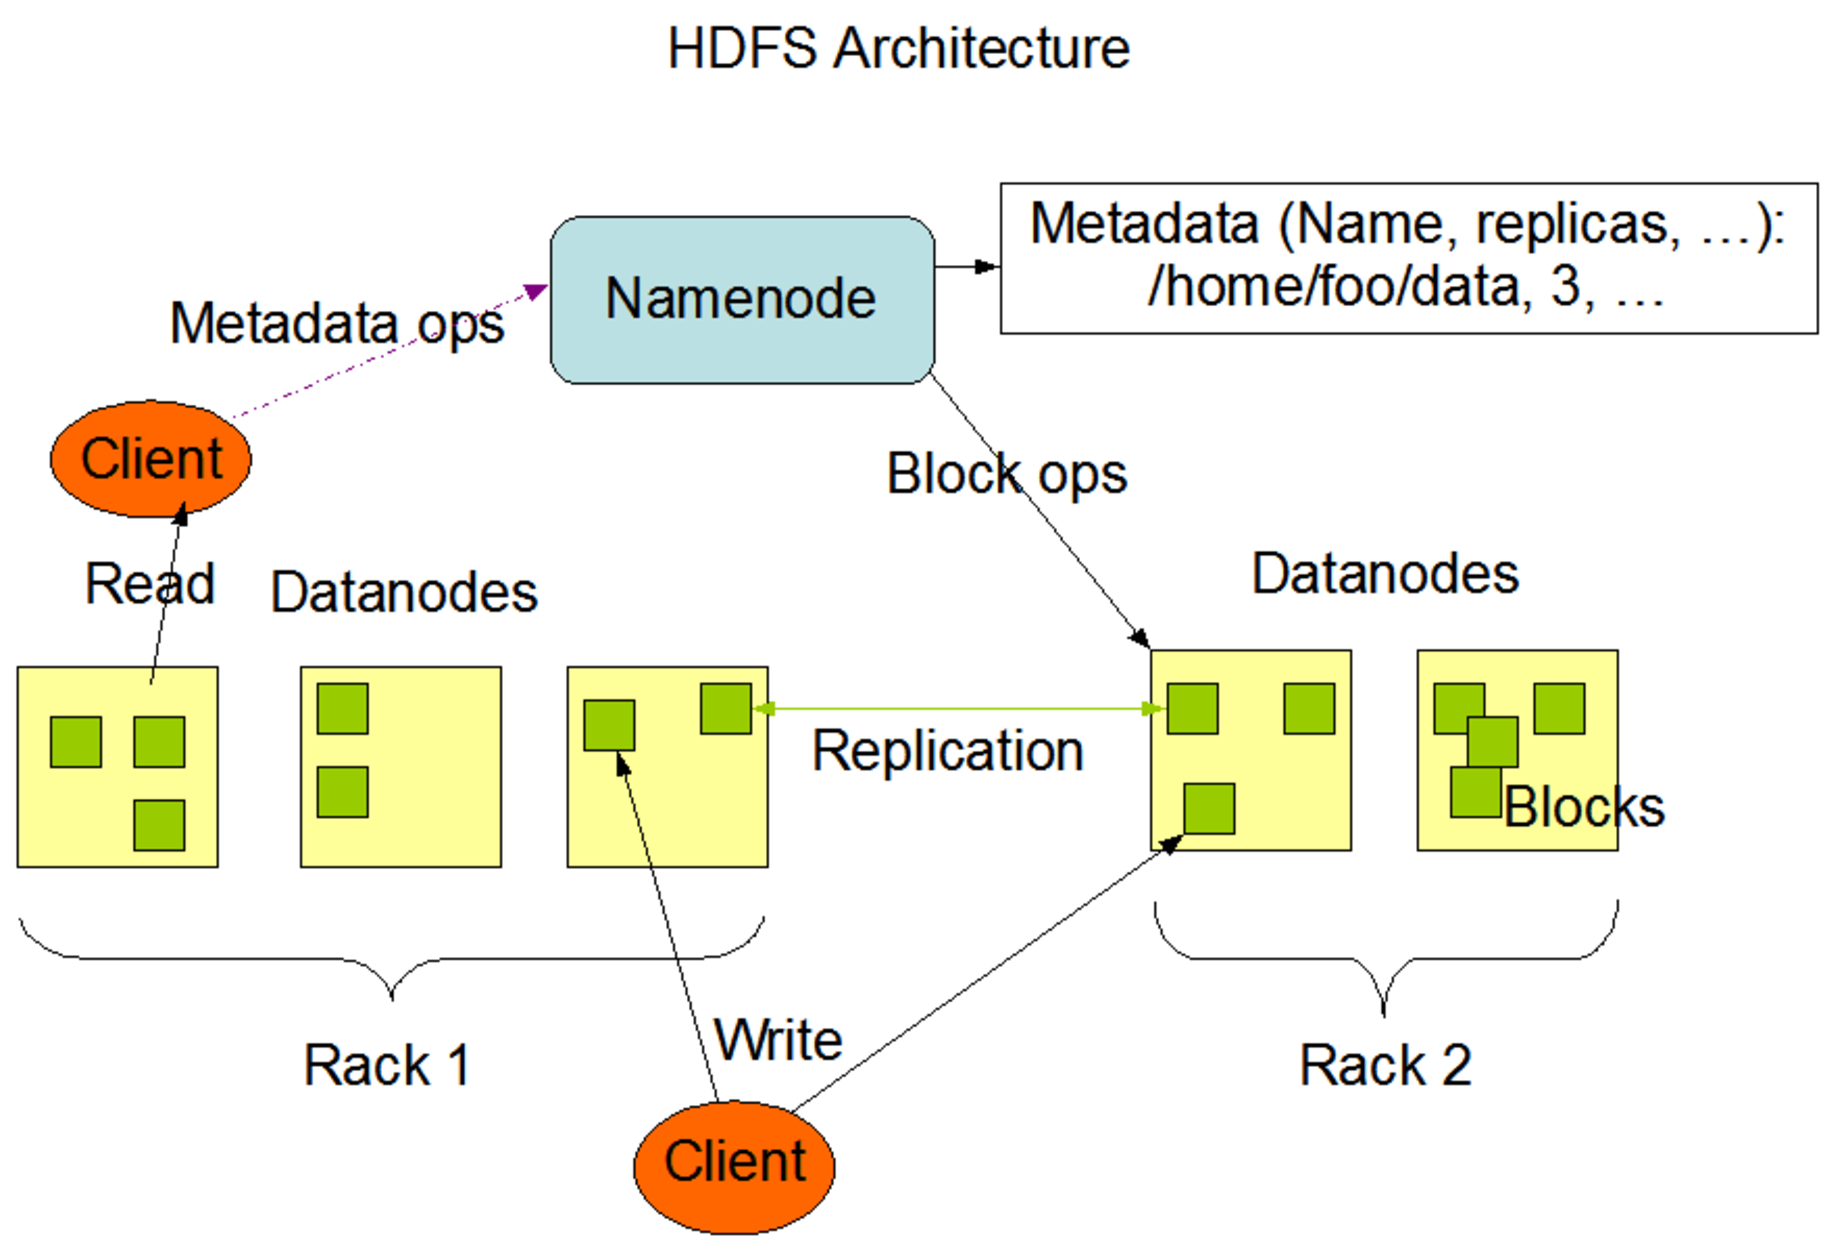
\includegraphics[scale=0.35]{images/hdfsarchitecture}}
   \caption{HDFS architecture \cite{HDFS}}
   \label{fig:hdfs_architecture}
  \end{center}
\end{figure}

Hadoop Distributed File System \cite{HDFS} is open source project of Google File System (GFS) \cite{ghemawat2003google} that is deployed on computing cluster. In following text of this thesis, we will use HDFS as its abbreviation. HDFS is highly fault-tolerant and is designed to be deployed on low-cost hardware. HDFS provides high throughput access to application data and is suitable for applications that have large data sets. HDFS relaxes a few POSIX requirements to enable streaming access to file system data. \cite{HDFS} The assumptions and goals of HDFS includes: hardware failure, high throughput, large dataset, streaming access, data load balance and simple coherency model, "Moving Computation is Cheaper than Moving Data", and portability across heterogeneous hardware and software platforms. 

An HDFS instance may consist of hundreds or thousands of nodes, each handling part of the file system's data. Therefore, HDFS could store very large dataset and provide high throughput. Normally, the failure probability of a machine is non-trivial. But in a cluster with thousands machines, some nodes would be always non-functional. From Figure~\ref{fig:hdfs_architecture} it is clear to know that HDFS architecture is master-slaves architecture with a namenode and multi datanodes. Based on this architecture, any crashed datanode can be checked out by sending heartbeat messages periodically to namenode. Once certain datanode fail to send heartbeat message to namenode within regulated time period, namenode would mark that datanode inactive and ask other datanodes to replicate data on the failed datanode. When free space on certain servers are below the threshold specified on the configuration file, other datanodes are also asked to replicate data on overhead datanode to achieve data load balance. HDFS applications need a write-once-read-many access model for files. A file once created, written, and closed need not be changed. This assumption simplifies data coherency issues and enables high throughput data access.\cite{HDFS} A computation is much more efficient if it is executed in the same node or near the node where the request data located. Because transmission of data takes much more time than changing a server to do a computation. Base on this assumption, HDFS provides interfaces for applications to move themselves closer to where the data is located. In addition, one more thing in the respect of fault tolerance is referred. The principle of fault tolerance in HDFS refers to checkpoint and then HDFS recovers data from checkpoint at certain time point when certain slave server is crashed down.

In general, HDFS and MapReduce always works together. In a distribute cluster, each datanode in HDFS runs  a TaskTracker as a slave node in MapReduce. MapReduce retrieves data from HDFS and executes computation and finally writes results back to HDFS.

\subsection{Kafka}
\begin{figure}
  \begin{center}
  \subfigure{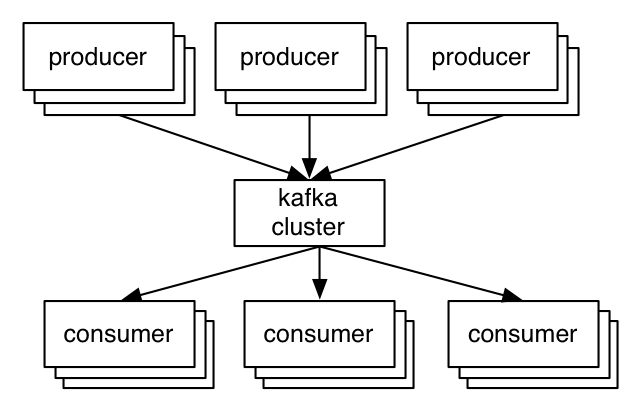
\includegraphics[scale=0.75]{images/kafka_producer_consumer}}
   \caption{Kafka producer and consumer \cite{Kafka}}
   \label{fig:kafka_producer_consumer}
  \end{center}
\end{figure}

ApacheKafka is a distributed, partitioned, replicated commit log service developed by the Apache Software Foundation. It aims to provide a unified, high-throughput, low-latency platform for handling real-time data feeds. Before we go into architecture of Kafak, there are some basic messaging terminologies: \cite{Kafka}

\begin{itemize}
  \item \textbf{Topic:} Kafka maintains feeds of messages in categories called topics. 
  \item \textbf{Producer:} Processes that publish messages to a Kafka topic are called producers.
  \item \textbf{Consumer:} Processes that subscribe to topics and process the feed of published messages are consumers.
   \item \textbf{Broker:} Kafka is run as a cluster comprised of one or more servers each of which is called a broker.
\end{itemize}

As Figure~\ref{fig:kafka_producer_consumer} shown, producers send messages over the network to the Kafka cluster which holds on to these records and hands them out to consumers. More specifically, producers publish their messages to a topic, and consumers subscribe to one or more topics. Each topic could have multiple partitions that are distributed over the servers in Kafka cluster, allowing a topic to hold more data than storage capacity of any server. Each partition is replicated across a configurable number of servers for fault tolerance. Each partition is an ordered, immutable sequence of messages that is continually appended to?a commit log. The messages in the partitions are each assigned a sequential id number called the offset that uniquely identifies each message within the partition.  Figure ~\ref{fig:kafka_partitioned_topic} shows a producer process appending to the logs for the two partitions, and a consumer reading from partitions sequentially. 

At a high-level Kafka gives the following guarantees: \cite{Kafka}
\begin{itemize}
  \item Messages sent by a producer to a particular topic partition will be appended in the order they are sent. That is, if a message M1 is sent by the same producer as a message M2, and M1 is sent first, then M1 will have a lower offset than M2 and appear earlier in the log. 
  \item A consumer instance sees messages in the order they are stored in the log.
  \item For a topic with replication factor N, we will tolerate up to N-1 server failures without losing any messages committed to the log.
\end{itemize}


Another very important feature of Kafka is messages with the same partition key will be sent to the same partition that is very important to our benchmark.
% kafka guarantees that data with same key will be sent to the same partition


\begin{figure}
  \begin{center}
  \subfigure{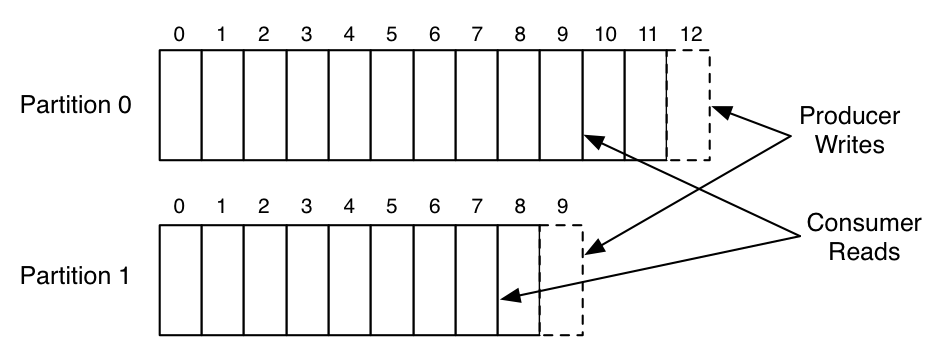
\includegraphics[scale=0.75]{images/partitioned_log}}
   \caption{Kafka topic partitions}
   \label{fig:kafka_partitioned_topic}
  \end{center}
\end{figure}
% \subsection{Zookeeper}
% ZooKeeper is a centralized service for maintaining configuration information, naming, providing distributed synchronization, and providing group services. All of these kinds of services are used in some form or another by distributed applications. Each time they are implemented there is a lot of work that goes into fixing the bugs and race conditions that are inevitable. Because of the difficulty of implementing these kinds of services, applications initially usually skimp on them ,which make them brittle in the presence of change and difficult to manage. Even when done correctly, different implementations of these services lead to management complexity when the applications are deployed.

\section{Benchmark}
Batch processing technologies(Such as MapReduce, Hive, Pig) have matured and been widely used in the industry. These systems solved the issue processing big volumes of data successfully. However, first big data need to be collected and stored in a database or file system. Then it takes time to finish batch processing analysis job before get any results. While there are many cases that need analysed results from streaming data immediately. The demand for processing real time stream data is increasing a lot these days. A big data architecture contains several parts. Often, masses of structured and semi-structured historical data are stored in Hadoop (Volume + Variety). On the other side, stream processing is used for fast data requirements (Velocity + Variety)\cite{GameChanger}. Several streaming processing systems are implemented and widely adopted, such as Apache Storm, JStorm, Apache Spark, IBM InfoSphere Streams and Apache Flink. They all support real-time stream processing, high scalability, and awesome monitoring. How to evaluate a real time stream processing system before choosing it to use in production development is a open question.  Before these real time stream processing systems are implemented, Michael demonstrated the 8 requirements \cite{8requirements} of real-time stream processing, which gives us a standard to evaluate whether a real time stream processing system satisfies these requirements.  A very common and traditional approach to verify whether the performance of a system meets the requirements is benchmarking. Published benchmarking results from industry standard benchmark systems could help users compare products and understand features of a system easily.

\subsection{Traditional Database Benchmarks}
Traditional database management systems were evaluated with industry standard benchmarks like TPC-C,  \cite{TPC-C} TPC-H. \cite{TPC-H} These have focused on simulating complete business computing environment where plenty of users execute business oriented ad-hoc queries that involve transactions, big table scan, join and aggregation. The queries and the data populating the database have been chosen to have broad industry-wide relevance. This benchmark illustrates decision support systems that examine large volumes of data, execute queries with a high degree of complexity, and give answers to critical business questions. \cite{TPC-H} The integrity of the data is verified during the process of the execution of the benchmark to check whether the DBMS corrupt the data. If the data is corrupted, the benchmark measurement is rejected entirely. \cite{dey2014ycsb+t} Benchmark systems for DBMS mature, with data and workloads simulating real common business use cases, they could evaluate performance of DBMS very well. Some other works were done related to specific business model. Linkbench \cite{LinkBench} benchmarks database systems which store "social network" data specifically. The workload of database operations are based on Facebook's production workload and the data is also generated in such a way that key properties of the data match the production social graph data in Facebook.  

\subsection{Cloud Service Benchmarks}
As the data size keep increasing, traditional database management systems could not handle some use cases with very big size data very well. To solve this issue, there are plenty of NoSql database systems developed for cloud data serving. With the widespread use of such cloud services, several benchmarks are introduced to evaluate these cloud systems.

One widely used and accepted extensible cloud serving benchmark named \textit{Yahoo! Cloud Servicing Benchmark}(YCSB) developed by Yahoo. \cite{YCSB} It  proposes two benchmark tiers for evaluating the performance and scalability of cloud data serving systems such as Cassandra, HBase and CouchDB. A core set of workloads are developed to evaluate different tradeoffs of cloud serving systems. Such as write/read heavy workloads to determine whether system is write optimised or read optimised. To evaluate transaction features in later NoSql database,  YCSB+T \cite{dey2014ycsb+t} extends YCSB with a specific workload for transaction called Closed Economy Workload(CEW). A validation phase is added to the workload executor to check consistency of these cloud databases. YCSB++ \cite{ycsb++} is another set of extensions of YCSB to benchmark other five advance features of cloud databases such as bulk insertions, server-side filtering. YCSB++ could run multiple clients on different machines that coordinated with Apache ZooKeeper, which increases test ability of benchmark framework. \citet{pokludabenchmarking}  explore the design and implementation of two representative systems and provide benchmark results using YCSB. In addition to the performance aspect of NoSql systems, they also benchmark availability and providing an analysis of the failover characteristics of each. \citet{Kuhlenkamp} made some contributions to benchmarking scalability and elasticity of two popular cloud database systems HBase and Cassandra. The benchmark strategy is changing workloads and/or system capacity between workload runs, load and/or system capacity are changed.

These efforts are island solutions and not policed by any industry consortia. BigBench aims to be implemented as an industry standard big data benchmark \cite{BigBench}. It is an end to end benchmark identify business levers of big data analytics. Inherit from TPC-DS benchmark, BigBench implements the complete use-case of a realistic retail business. The data model of which covers three major characteristics described by \citet{laney20013d} of big data system: volume(larger data sizes), velocity(higher data arrive rates) and variety(increased data type disparity). The main part of the workload is the set of queries to be executed against the data model. These queries are designed along one business dimension and three technical dimensions. \cite{BigBench}

\subsection{ Distributed Graph Benchmarks}

A specific type of big data which keeps increasing in day-to-day business is graph data. The growing scale and importance of graph data has driven the development of numerous specialized graph processing systems including Google's proprietary Pregel system \cite{Pregel}, and Apache Giraph \cite{Giraph}, PowerGraph\cite{PowerGraph}. In the paper, \citet{guo2014benchmarking} demonstrate the diversity of graph-processing platforms and challenges to benchmark graph-processing platforms. Among these challenges, some are common for general benchmark systems, such as evaluation process, dataset selection and result reporting. To address these issues of evaluating graph-processing platforms, \citeauthor{guo2014well} implemented a benchmark suit using an empirical performance-evaluation method which includes four stages: identifying the performance aspects and metrics of interest; defining and selecting representative datasets and algorithms; implementing, configuring, and executing the tests; and analyizing the results. In order to create an industry-accepted benchmark, this method still raises some issues. In latest released papers\cite{iosup2014towards, capota2015graphalytics}, the team implemented a benchmark called Graphalytics for graph-processing platforms. 

\subsection{ Existing stream processing benchmarks}

To help users have a better understanding of stream processing system and choose one intelligently in practical work, there are already several tests or benchmarks of stream processing systems published on the Internet. Early work by \citet{cordovaanalysis} focuses on analysing performance of two notable real time stream systems Spark streaming and Storm Trident. While it could not be a standard benchmark because it is not extensible and experiment cluster is too small with only 3 nodes. More ever, the data model and workloads are quite simple which could not reflect the real use cases in business. IBM compares the performance of IBM InfoSphere Streams against Apache Storm with a real-world stream processing application detect online spam. \cite{ibm2014streams} The processing pipeline for the benchmark email classification system is divided into 7 stages and implemented by InfoSphere Streams and Apache Storm separately. The main drawback of this approach is there is only one scenario. First, the workload includes different steps(operations) makes it hard to detect the possible performance bottleneck. There are some other features of Streams and Storm that are not included in the application such as sort. \citet{xinhstechblog} in her blog compared Storm and Spark Streaming side-by-side, including processing model, latency, fault tolerance and data guarantees. LinkedIn benchmarked its own real-time streaming process system Samza running four simple jobs and got excellent performance: 1.2 million messages per second on a single node \cite{samza-benchmark}. Other similar works \cite{manoj-sotrm-vs-spark,flink-latency} are all focusing on compare two or three specific real-time streaming process systems. Recently, Yahoo Storm Team demonstrated a stream processing benchmark. Design and more features of \textit{The Yahoo Streaming Benchmark} will be introduced in detail in the next section.

\subsection{The Yahoo Streaming Benchmark}
\begin{figure}
  \begin{center}
  \subfigure{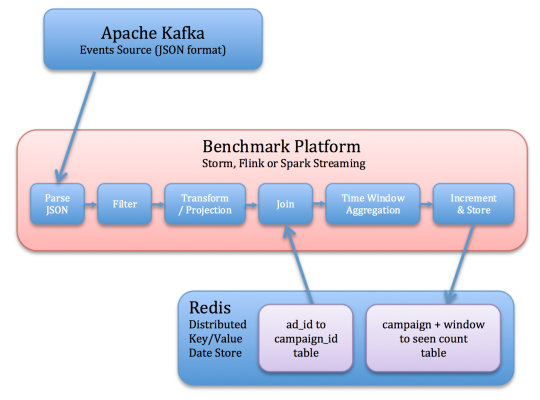
\includegraphics[scale=0.50]{images/yahoo_stream_bench}}
   \caption{Operations flow of YSB \cite{YSB}}
   \label{fig:yahoo_stream_bench}
  \end{center}
\end{figure}


The Yahoo Streaming Benchmark(YSB) is introduced to analysis what Storm is good at and where it needs to be improved compared to other stream processing systems by Yahoo Strom Team. \cite{YSB} The benchmark is a single advertisement application to identify relevant advertisement events. There are a number of advertising campaigns, and a number of advertisements for each campaign. The application need read various JSON events from a Kafka topic, identify the relevant events, and store a windowed count of relevant events per campaign into Redis. The flow of operations could be shown as Figure~\ref{fig:yahoo_stream_bench}.

Each event(message) in Kafka topic contains a timestamp marking the time producer created this event. Truncating this timestamp to a particular digit gives the begin-time of the time window that the event belongs in. When each window is updated in Redis, the last updated time is recored.

After each run, a utility reads windows from Redis and compares the windows? times to their last update times in Redis, yielding a latency data point. Because the last event for a window cannot have been emitted after the window closed but will be very shortly before, the difference between a window?s time and its last update time minus its duration represents the time it took for the final tuple in a window to go from Kafka to Redis through the application. \\

$finalEventLatency = (lastUpdatedTime - timestamp) - duration$ \\

More details about how the benchmark setup and the configuration of experiment environment could be found here~\footnote{\url{http://yahooeng.tumblr.com/post/135321837876/benchmarking-streaming-computation-engines-at}}. From experiments demonstrated in this page, Storm 0.10.0 was not able to handle throughputs above 135,000 events per second. The larget rate at which Kafka emitted data events into the Flink benchmark is varied 170,000 events/sec which doesn't reach throughput of Flink. From the design and conclusion of experiments, it is very obvious that the benchmark focus more on latency other than throughput of stream processing systems. Another shortage of this benchmark is one single workload could not reflect features of stream processing systems comprehensively, even the steps of benchmark flow attempt to probe common operations performed on data streams.


\clearpage


\chapter{Stream Processing Platforms}
Introduce three widely used stream processing platforms, point out core concepts and key features 

\section{Apache Storm}
\subsection{Storm Architecture}
\subsection{Computing Model}

\section{Apache Flink}
\subsection{Flink Architecture}
\subsection{Memory Management}
\subsection{Flink Streaming}


\section{Apache Spark}
\subsection{ Resilient Distributed Datasets(RDDs)}
\subsection{Spark Streaming}

\section{Other Stream Processing Systems}
\subsection{Amazon S4}
\subsection{Apache Samaza}
\subsection{Apache Apex}
\subsection{Aurora}
\clearpage

\chapter{Benchmark Design}
We developed a tool, called StreamBench, to execute benchmark workloads on stream processing systems. A key feature of StreamBench is extensibility, so that it could be extended not only to run new workloads but also to benchmark new stream processing systems. We have used StreamBench to measure the performance of several stream processing systems, as we report in the next chapter.  StreamBench is also available under an open source license, so that others may use and extend it, and contribute new workloads and stream processing system interfaces.

This chapter illustrates the architecture of StreamBench and introduce more detail of main components of StreamBench. 

\section{Architecture}

\begin{figure}
  \begin{center}
  \subfigure{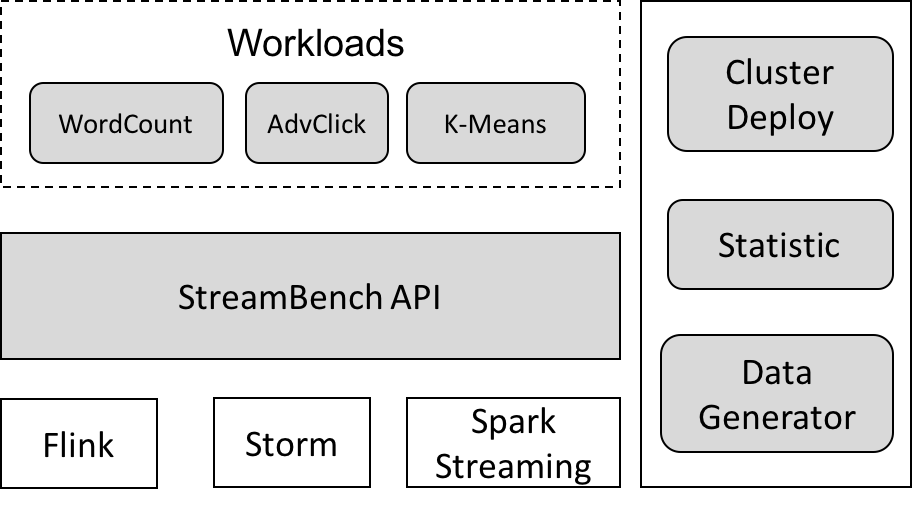
\includegraphics[scale=0.6]{images/benchmark_architecture}}
   \caption{StreamBench architecture}
   \label{fig:streambench_architecture}
  \end{center}
\end{figure}

The main component of StreamBench is a Java program for consuming data from partitioned kafka topic and executing workloads on stream processing cluster. The architecture of StreamBench is shown in Figure~\ref{fig:streambench_architecture}. The core of the architecture is StreamBench API which contains several states of stream and a set of stream processing APIs what are very similar to Flink's computational model. For example, API \texttt{mapToPair} maps a normal data stream to a keyed data stream, and API \texttt{filter} is a method with a parameter of boolean function and evaluates this boolean function for each element and retains those for which the function returns true. 

StreamBench API could be engined by different stream processing systems. Currently we support these APIs on three stream processing systems: Storm, Flink and Spark Streaming. It is very convenient to implement most interfaces of StreamBench API on Flink and Spark Streaming which have similar high level APIs. But there are also some APIs that Flink and/or Spark Streaming doesn't support well. For example, currently, Flink \texttt{join} operator only supports two streams joining on the same size window time. Therefore, we implemented another version \texttt{join} operator discussed in ~\cref{sub:join_operator} with Flink's low level API. Compare to Flink and Spark Streaming, Storm is more flexible by providing two low level APIs: spout and bolt. Bolts represent the processing logic unit in Storm. One can utilize bolts to do any kind of processing such as filtering, aggregating, joining, interacting with data stores, talking to external systems etc.

With these common stream processing APIs, we implemented three workloads to benchmark performance of stream processing systems in different aspects. WordCount discussed in~\cref{sub:basic_operator} aims to evaluate the performance of stream processing systems performing basic operators. In~\cref{sub:join_operator}, we demonstrated a workload named AdvClick to benchmark two keyed streams joining operation. To check the performance of iterate operator, we designed a workload to calculate k-means of a point stream. More detail of this workload could be found in~\cref{sub:iterate_operator}.

Except the core Java program, the architecture also includes three more components: Cluster Deploy, Data Generator and Statistic. Section~\ref{chapter:environment_setup} illustrates how to use cluster deploy scripts to setup experiment environment. Data generators generate test data for workloads and send it to kafka cluster that is demonstrated detailedly in ~\cref{section:data_generator}. The Statistic component discussed in ~\cref{section:log_statistic} includes experiment logging and performance statistic. 


\section{Experiment Environment Setup}
\label{chapter:environment_setup}

The experiment environment is a cloud service called cPouta which is the main production IaaS cloud at CSC -- a non-profit, state-owned company administered by the Ministry of Education and Culture. In cPouta,  there are several available virtual machine flavors. Each visual machine used in our experiment has 4 CPU cores, 15GB RAM, 10GB root disk and 220GB ephemeral disk. The experiment environment consists of two clusters: compute cluster and Kafka cluster. Computer cluster consists of 8 work nodes and one master nodes. Kafka cluster has 5 brokers with one zookeeper instance running on the same machine with one Kafka broker. The cPouta service is based on the hardware of the Taito cluster. Communication among nodes and to the storage is done by Infiniband FDR fabric, which provides low latency and high throughput connectivity. The detail information about hardware and inter connection could be found online~\footnote{\url{https://research.csc.fi/taito-supercluster\#1.1.2}}.

The operating system running on experiment nodes is Ubuntu 14.04 LTS. Benchmarked stream processing systems are Spark-1.5.1, Storm-0.10.0 and Flink-0.10.1. To enable checkpoint feature of Spark, Hadoop2.6(HDFS) is installed in compute cluster. Kafka 0.8.2.1 is running as distribute message system here. 

To deploy these software in compute cluster and kafka cluster automatically, we developed a set of python script. The prerequisites of using these scripts include internet access, ssh passwordless login between nodes in cluster and cluster configuration that describes which nodes are compute node or kafka node and where is the master node. The basic logic of deploy scripts is to download softwares online and install them, then replace configure files which are contained in a Github repository. For detail information of how to use cluster deploy scripts and configure of Storm, Flink, Spark and Kafka, please check this Github repository~\footnote{\url{https://github.com/wangyangjun/StreamBench}}.

\section{Workloads}
\label{section:workloads}

In StreamBench, a workload consists of a stream processing application and one or more kafka topics. The application consumes messages from kafka cluster and executes operations or transformations on the messages. We have developed 3 workloads to evaluate different aspects of a system's performance. Each workload contains a representative operation or feature of stream processing system that can be used to evaluate systems at one particular point in the performance space. We have not attempted to exhaustively examine the entire performance space. As StreamBench is open sourced, users could also defined their own workloads either by defining a new set of workload parameters, or if necessary by implement a new workload which is discussed detailedly in~\cref{section:extensibility}.


\subsection{Basic Operators}
\label{sub:basic_operator}

With the widespread use of computer technologies, there is an increasing demand of processing unbounded, continuous input streams. In most cases, only basic operations need to be performed on the data streams such as \texttt{map}, and \texttt{reduce}. One good sample is stream WordCount. WordCount is a very common sample application of Hadoop MapReduce that counts the number of occurrences of each word in a given input set\cite{MapReduce}. Similarly, many stream processing systems also support it as an sample application to count words in a  given input stream. Stream WordCount is implemented with basic operations which are supported by almost all stream processing systems. It means either the system has such operations by default or the operations could be implemented with provided built-in APIs. Other basic operations include \texttt{flatMap}, \texttt{mapToPair} and \texttt{filter} which are similar to \texttt{map} and could be implemented by specializing \texttt{map} if not supported by default. The pseudocode of WordCount implemented with StreamBench APIs could be abstracted as Algorithm~\ref{alg:word_count}.

\begin{algorithm}
\caption{WordCount}\label{euclid}
\label{alg:word_count}
\begin{algorithmic}[1]
\State $\textit{sentenceStream.flatMap(...)}$
\State \hspace{2.6cm} $\textit{.mapToPair(...)}$
\State \hspace{2.6cm} $\textit{.reduceByKey(...)}$
\State \hspace{2.6cm} $\textit{.updateStateByKey(...)}$

\end{algorithmic}
\end{algorithm}

One special case of the basic APIs is \texttt{updateStateByKey}. Only in Spark Streaming there is a corresponding built-in operation. As discussed in Section~\ref{section:spark}, the computing model of Spark Streaming is micro-batch which is different with that of other stream processing systems. The results of operation \texttt{reduceByKey} of WordCount running in Spark Streaming is word counts of one single micro batch data set. Operation \texttt{updateStateByKey} is used to accumulate word counts in Spark Streaming. Because the model of Flink and Storm is stream processing and accumulated word counts are returned from \texttt{reduceByKey} directly. Therefore, when implementing the API \texttt{updateStateByKey} with Flink and Storm engine, nothing need to do. 

% window pre-aggregation
When dealing with skewed data, the compute node which count the word with largest frequency might be the bottleneck. Inspired from MapReduce Combiner, we designed another version of WordCount with \texttt{window} operator of stream processing. Windows are typically groups of events within a certain time period. In the reduce step of Windowed WordCount, first words are shuffle grouped and applied pre-aggregation. In a certain time period, local pre-aggregation results are stored at local compute nodes. At the end of a window time, the intermedia word counts are key grouped and reduced to get the final results.

%The goal of this workload is to evaluate the performance of stream processing systems executing basic operations.  
\begin{figure}
  \begin{center}
  \subfigure{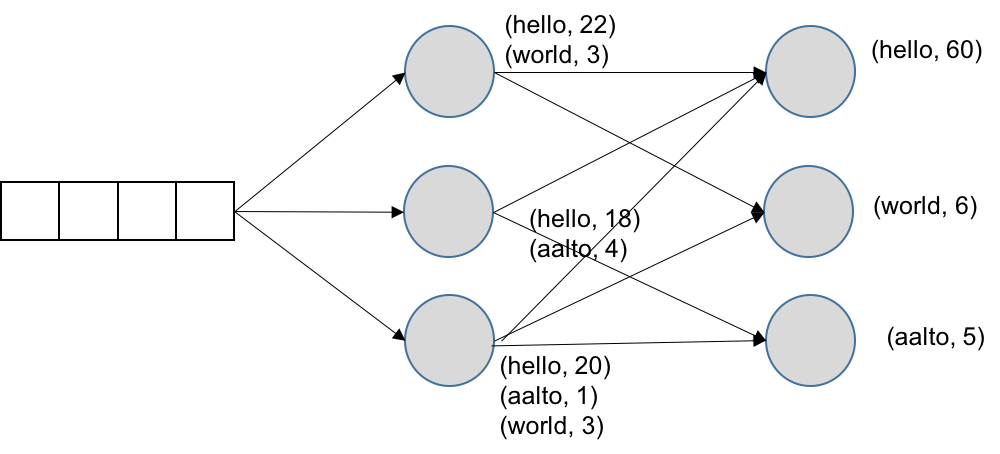
\includegraphics[scale=0.4]{images/window_wordcount}}
   \caption{Windowed WordCount}
   \label{fig:windowed_wordcount}
  \end{center}
\end{figure}


\subsection{Join Operator}
\label{sub:join_operator}

Besides the cases in which only basic operations are performed, another typical type of stream use case is processing joins over two input streams. For example, in a surveillance application, we may want to correlate cell phone traffic with email traffic. Theoretically unbounded memory is required to processing join over unbounded input streams, since every record in one infinite stream must be compared with every record in the other. Obviously, this is not practical\cite{window-join}. Since the memory of a machine is limited, we need restrict the number of records stored for each stream with a time window. 

A window join takes two key-value pair streams, say stream \textit{S1} and stream \textit{S2}, along with windows with the same slide size for both \textit{S1} and \textit{S2} as input. Each record in \textit{S1} is a tuple of pair \texttt{(k, v1)} with \texttt{k} as the primary key. The key in Stream \textit{S2:}\texttt{(k, v2)} is a foreign key referencing primary key in \textit{S1}. The output of join operator is a stream of tuple \texttt{(k, v1, v2)}. This primary key join operation could be described as a SQL query illustrated in Algorithm~\ref{alg:join_query}. Assuming a sliding window join between stream \textit{S1} and stream \textit{S2}, a new tuple arrival from stream \textit{S2}, then a summary of steps to preform join is the following:

\begin{algorithm}
\caption{Join Query}\label{euclid}
\label{alg:join_query}
\begin{algorithmic}[1]
\State SELECT $\textit{S1.k},  $\textit{ S1.v1},  $\textit{S2.v2}$
\State FROM $\textit{S1}$
\State INNER JOIN $\textit{S2}$
\State ON $\textit{S1.k}$ =  $\textit{S2.k}$
\end{algorithmic}
\end{algorithm}

\begin{enumerate}
\item Scan window of stream \textit{S1} to find any tuple which has the same key with this new tuple and propagate the result;
\item 
\begin{enumerate}
\item Invalidate target tuple in stream \textit{S1}'s window if found ;
\item If not, insert the new tuple into stream \textit{S2}'s window 
\end{enumerate}
\item Invalidate all expired tuples in stream \textit{S2}'s window.
\end{enumerate}

\begin{figure}
  \begin{center}
  \subfigure{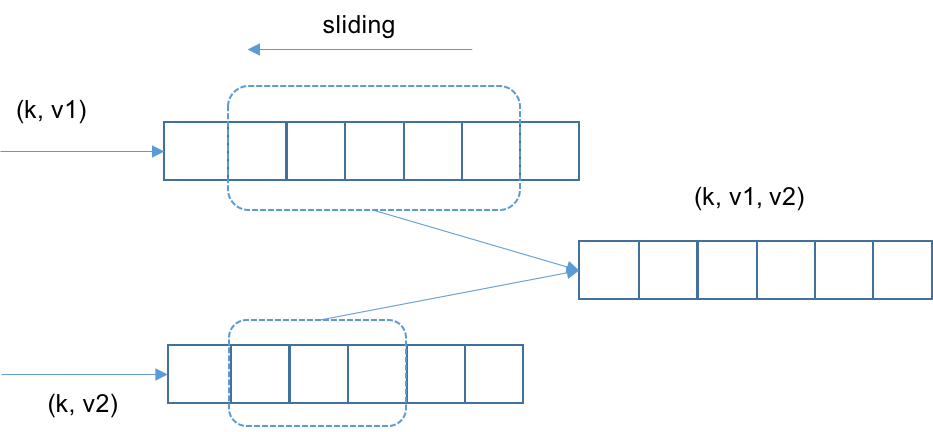
\includegraphics[scale=0.6]{images/join}}
   \caption{Window join scenario}
   \label{fig:window_join}
  \end{center}
\end{figure}

Every time new tuple arrives stream \textit{S2}, window of stream \textit{S1} need be scanned. That reduces the performance of join operation, especially when the window is big. With a data structure named \texttt{cachedHashTable} there is another way to implement stream join. The tuples in the window of a stream are stored in a cached hash table. Each tuple is cached for window time and expired tuples are invalidated automatically. One of such a \texttt{cachedHashTable} could be found in Guava.\footnote{\url{http://docs.guava-libraries.googlecode.com/git/javadoc/com/google/common/cache/CacheBuilder.html}} Instead of scanning window of stream \textit{S2}, we could find tuple with the same key in \textit{S2} directly by calling \texttt{cachedHashTable.get(k)}. In theory, this implementation achieves better performance. 

Since Spark Streaming doesn't process tuples in a stream one by one, the join operator in Spark Streaming has different behaviours. In each batch interval, the RDD generated by stream1 will be joined with the RDD generated by stream2. For windowed streams, as long as slide durations of two windowed streams are the same, in each slide duration, the RDDs generated by two windowed streams will be joined. Because of this, window join in Spark Streaming could only make sure that a tuple in one stream will always be joined with corresponding tuple in the other stream that arrived earlier up to a configureable window time. Otherwise, repeat joined tuples would exist in generated RDDs of joined stream. As Figure~\ref{fig:spark_join_norepeat} shown, a tuple in Stream2 could be always joined with a corresponding tuple in Stream1 that arrived up to 2 seconds earlier. Since the slide duration of Stream2 is equal to its window size, no repeat joined tuple exists. On the other hand, it is possible that a tuple arrives earlier from Stream2 than the corresponding tuple in Stream1 couldn't be joined. Figure~\ref{fig:spark_join_repeat} exemplifies that there are tuples joined repeatedly  when slide duration of Stream2 is not equal to its window size.

\begin{figure}
  \begin{center}
  \subfigure{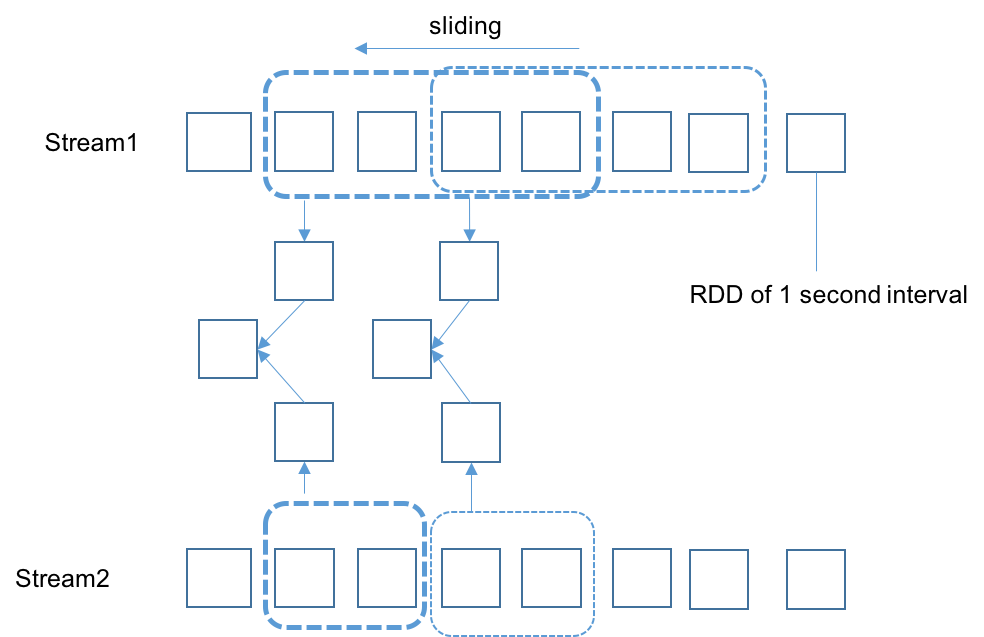
\includegraphics[scale=0.6]{images/spark_join_norepeat}}
   \caption{Spark Stream join without repeated tuple}
   \label{fig:spark_join_norepeat}
  \end{center}
\end{figure}


To evaluate performance of join operator in stream processing systems, we designed a workload called AdvClick which joins two streams in a online advertisement system. Every second there are a huge number of web pages opened which contain advertisement slots. A corresponding stream of shown advertisements is generated in the system. Each record in the stream could be simply described as a tuple of \texttt{(id, shown time)}. Some of advertisements would be clicked by users and clicked advertisements is a stream which could be abstracted as a unbounded tuples of \texttt{(id, clicked time)}. Normally, if an advertisement is attractive to a user, the user would click it in a short time after it is shown. We call such a click of an attractive advertisement valid click. To bill a customer, we need count all valid clicks regularly for advertisements of this customer. That could be counted after joining stream \texttt{advertisement clicks} and stream \texttt{shown advertisements}. 

\begin{figure}
  \begin{center}
  \subfigure{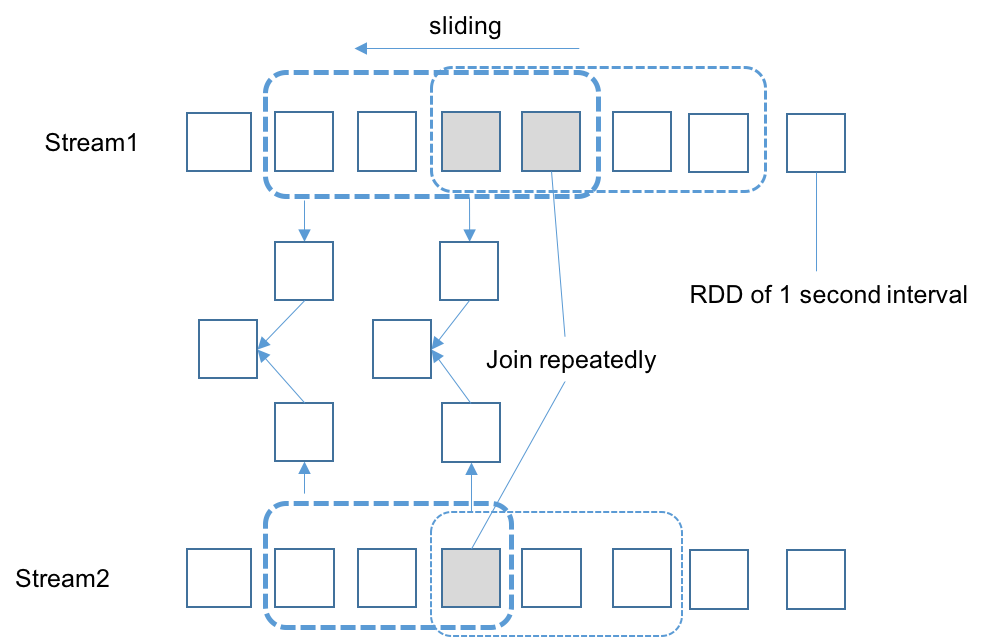
\includegraphics[scale=0.6]{images/spark_join_repeat}}
   \caption{Spark Stream join with repeated tuples}
   \label{fig:spark_join_repeat}
  \end{center}
\end{figure}

\subsection{Iterate Operator}
\label{sub:iterate_operator}

Iterative algorithms occur in many domains of data analysis, such as machine learning or graph analysis. Many stream data processing tasks require iterative sub-computations as well. These require a data processing system having the capacity to perform iterative processing on a real-time data stream. To achieve iterative sub-computations,  low-latency interactive access to results and consistent intermediate outputs, \citeauthor{murray2013naiad} introduced a computational model named timely dataflow that is based on a directed graph in which stateful vertices send and receive logically timestamped messages along directed edges \cite{murray2013naiad}. The dataflow graph may contain nested cycles and the timestamps reflect this structure in order to distinguish data that arise in different input epochs and loop iterations. With iterate operator, many stream processing systems already support such nested cycles in processing data flow graph. We designed a workload named stream k-means to evaluate iterate operator in stream processing systems.

K-means is a clustering algorithm which aims to partition n points into k clusters in which each point belongs to the cluster with the nearest mean, serving as a prototype of the cluster\cite{kmeans_wiki}. Given an initial set of k means, the algorithm proceeds by alternating between two steps\cite{mackay2003information}:
\begin{description}
\item\textbf{Assignment step:} assign each point to the cluster whose mean yields the least within-cluster sum of squares.
\item \textbf{Update step:} Calculate the new means to be the centroids of the points in the new clusters.
\end{description}

The algorithm has converged when the assignments no longer change. We apply k-means algorithm on a stream of points with an iterate operator to update centroids.

Compared to clustering for data set, the clustering problem for the data stream domain is difficult because of two issues that are hard to address: (1) The quality of the clusters is poor when the data evolves considerably over time. (2) A data stream clustering algorithm requires much greater functionality in discovering and exploring clusters over different portions of the stream\cite{aggarwal2003framework}. Considering the main purpose of this workload is to evaluate iterative loop in stream data processing, we don't try to solve these issues here. Similarly, stream k-means also has two steps: assignment and update. The difference is each point in the stream only passes the application once and the application doesn't try to buffer points. As shown in Figure~\ref{fig:iterator_operator}, once a new centroid calculated, it will be broadcasted to assignment executors. 

 \begin{figure}
  \begin{center}
  \subfigure{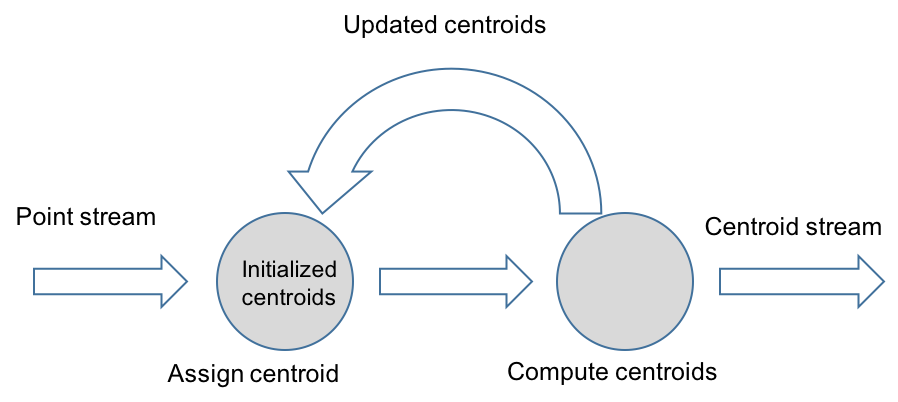
\includegraphics[scale=0.6]{images/iterator_operator}}
   \caption{Stream k-means scenario}
   \label{fig:iterator_operator}
  \end{center}
\end{figure}

Spark executes data analysis pipeline using directed acyclic graph scheduler.  Nested cycle doesn't exist in the data pipeline graph. Therefore, this workload will not be used to benchmark Spark Streaming. Instead, a standalone version of k-means application is used to evaluate the performance of Spark Streaming.

\section{Data Generators}
\label{section:data_generator}
 A data generator is a program that produces and sends unbounded records continuously to kafka cluster which are consumed by corresponding workload. For each workload, we designed one or several data generators with some configureable parameters which define the skew in record popularity, the size of records, and the distribution of data etc. These parameters could be changed to evaluate the performance of a system executing one workload on similar data streams with different properties. Users of StreamBench also could implement their own data generators to produce benchmarking data. Data generators are defined in a submodule of StreamBench project named \textit{generator}. The submodule could be compiled and packaged to get a jar file that could run on any node of our kafka cluster. 

\subsection{WordCount}
\label{subsection:wordcount_generator}

A data generator of workload WordCount produces unbounded lists of sentences, each sentence consists of several words. In StreamBench, we have implemented two versions of WordCount data generator. Each word in both generators is a 5-digit zero-padded string of a binary integer,  such as ``00001". The number of words in each sentence satisfies normal distribution with mean and sigma configured as \texttt{(10, 1)}. The difference between these two generators is the corresponding integers satisfy two different distributions: uniform distribution and zipfian distribution. Both uniform distribution and zipfian distribution have the same size -- 10000. Exponent of zipfian distribution is configured as 1. 

There are two different ways to run WordCount data generators to cooperate experiments of WordCount discussed in \cref{section:wordcount_experiment}. For Online WordCount, we start data generation after benchmark program and pass a parameter when starting generator to control the generation speed. For Offline model, we could either preload data to kafka cluster or make the generation speed much faster than the throughput of stream processing system executing WordCount workload.

\subsection{AdvClick}
\label{subsection:advclick_generator}

As discussed in Section~\ref{sub:join_operator}, workload AdvClick performs join operator on two streams: \texttt{shown advertisements} and \texttt{advertisement clicks}. Each record in  \texttt{shown advertisements} is a tuple consist of a universally unique identifier(\textbf{UUID}) and a timestamp. Each advertisement has a probability to be clicked, which is set to 0.3 in our experiments. Then the data generator could be a multi-threads application with main thread producing advertisements and sub-threads generating clicks. The pseudocode of the main thread is shown as Algorithm \ref{alg:advclick_generator}. After a sub-thread starts, it sleeps for delta time and then sends click record to corresponding kafka topic. The probability of advertisements click is a configureable parameter. In our experiments, mean of click delay is set to 10 seconds. 

\begin{algorithm}
\caption{AdvClick data generator}
\label{alg:advclick_generator}
\begin{algorithmic}[1]
\State $\text{load } \textit{clickProbability} \text{ from configure file}$

\State $\textit{cachedThreadPool} \gets \text{new CachedThreadPool}$
\State $\textit{dataGenerator} \gets \text{new RandomDataGenerator}$ 
\State $\textit{producer} \gets \text{new KafkaProducer}$ 

\While{not interrupted}
\State $\textit{advId} \gets \text{new UUID}$ 
\State $\textit{timestamp} \gets \text{current timestamp}$ 
\State $\textit{producer.send(...)}$ 

\If {$\textit{generator.nextUniform(0,1)} < clickProbability$} 
\State $\textit{deltaTime} \gets \textit{generator.nextGaussian(...)}$ 
\State $\textit{cachedPool.submit(new ClickThread(advId, daltaTime))} $ 
\EndIf
\EndWhile
\end{algorithmic}
\end{algorithm}

\subsection{KMeans}

Stream k-means is a one-pass clustering algorithm for stream data. In this workload, it is used to cluster a unbounded stream of points. The data generator produces such a stream of points. In order to make experiment results checking easy, we use pre-defined centroids. First, a set of centers are generated and written to a external file. There is a minimum distance between every two centers so that no two clusters are overlapped together. Then the generator produces points according these centers as Algorithm~\ref{alg:kmeans_generator}. The distance of each point to corresponding center satisfies normal distribution with mean and variance as configurable parameters. In our experiments, we found that random initial centroids would lead to results that two groups points cluster to a centroid which is in the middle of two real centers. Which is not desired output to measure the speed of convergence. Therefore, we generate initial centroids for each cluster in the same way as points generation.  

\begin{algorithm}
\caption{KMeans data generator}\label{euclid}
\label{alg:kmeans_generator}
\begin{algorithmic}[1]
\State $\text{load } \textit{covariances} \text{ from configure file}$
\State $\textit{means} \gets \text{original point}$
\State $\text{load } \textit{centroids} \text{ from external file}$

\State $\textit{producer} \gets \text{new KafkaProducer}$ 
\State $\textit{normalDistributon } \gets \text{ new NormalDistribution(means, converiances)}$

\While{not interrupted}
\State $\textit{centroid} \gets \text{pick a centroid from \textit{centroids} randomly}$ 
\State $\textit{point} \gets \textit{centroid+normalDistributon.sample()}$ 
\State $\textit{producer.send(point)}$ 

\EndWhile
\end{algorithmic}
\end{algorithm}

In our experiment environment, the compute cluster consists of 8 work nodes, each work node has 4 cpu cores. The parallelism of the compute cluster is 32. In order to have a better workload balance, we set the number of centers as 96. The dimension of point is configurable that enables to evaluate whether computation is a bottleneck of this workload.

\section{Experiment Logging and Statistic}
\label{section:log_statistic}

For evaluating the performance, there are two performance measurement terms used in StreamBench that are latency and throughput. Latency is the required time from a record entering the system to some results produced after some actions performed on the record. In StreamBench, messaging system and stream processing system are combined together and treated as one single system. The latency is computed start from when a record is generated. As discussed in Section \ref{section:data_generator}, data is sent to kafka cluster immediately after generation. Figure~\ref{fig:latency} shows how latency computed in StreamBench. In our experiments, we noticed that in the beginning of processing data, the performance of Storm cluster is bad. That leads to high latency of records in the head of a stream. Therefore, we ignored latency logs of first 1 minute in our statistic.

Throughput is the number of actions executed or results produced per unit of time. In the WordCount workload, throughput is computed as the number of words counted per seconds in the whole compute cluster. Joined click events and the number of points processed per second are the throughput of workloads AdvClick and Stream KMeans respectively.

There is an inherent tradeoff between latency and throughput: on a given hardware setup, as the amount of load increases by increase the speed of data generation, the latency of individual records increases as well since there is more contention for disk, CPU, network, and so on. Computing latency start from records generated makes it easy to measure the highest throughput, since records couldn't produced in time will stay in kafka topics that increase latency dramatically. A stream processing system with better performance will achieve low latency and high throughput with fewer servers.

\begin{figure}
  \begin{center}
  \subfigure{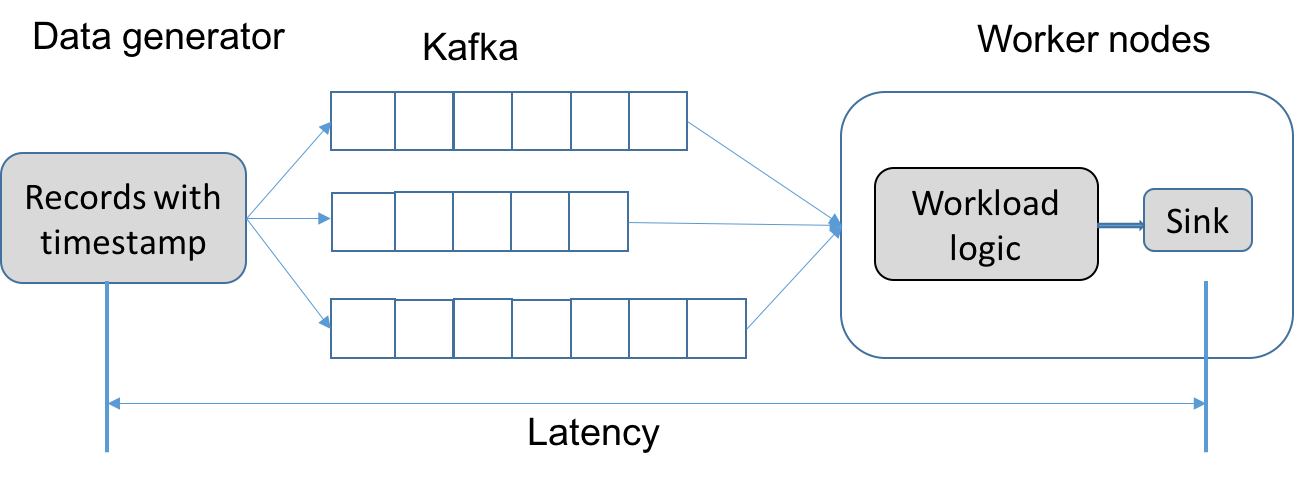
\includegraphics[scale=0.5]{images/latency}}
   \caption{Latency}
   \label{fig:latency}
  \end{center}
\end{figure}

\section{Extensibility}
\label{section:extensibility}

One significant feature of StreamBench is extensibility. The component "Workloads" in Figure~\ref{fig:streambench_architecture} contains three predefined workloads discussed in Section~\ref{section:workloads} that are implemented with common stream processing APIs. First, with some configuration modification of a data generator, which allows user to vary the skew in record popularity, and the size and number of records. The performances of a workload processing data streams with different properties could be different a lot. Moreover, it is easy for developers to design and implement a new workload to benchmark some specific features of stream processing systems. This approach allows for introducing more complex stream processing logic, and exploring tradeoffs of new stream processing features; but involves greater effort compared to the former approach.

Besides implementing new workloads, StreamBench also could be extended to benchmark new stream processing systems by implement a set of common stream processing APIs. A few samples of APIs could be shown as following:
\begin{itemize}
\item \textbf{map}(MapFunction\textless \textbf{T}, \textbf{R}\textgreater fun, String componentId): map each record in a stream from type \textbf{T} to type \textbf{R}
\item \textbf{mapToPair}(MapPairFunction\textless \textbf{T, K, V}\textgreater fun, String componentId): map a  item stream\textbf{\textless T\textgreater } to a pair stream\textbf{\textless K, V\textgreater}
\item \textbf{reduceByKey}(ReduceFunction\textless \textbf{V}\textgreater fun, String componentId): called on a pair stream of (\textbf{K, V}) pairs, return a new pair stream of (\textbf{K, V}) pairs where the values for each key are aggregated using the given reduce function
\end{itemize}

These methods are quite simple, representing common data transformations. There are some other APIs like \texttt{filter()}, \texttt{flatMap()} and \texttt{join} which are also easily to implement and supported well by most stream processing systems. Despite its simplicity, this API maps well to the native APIs of many of the stream processing systems we examined.







\section{Experiment}
\label{chapter:experiment}

\subsection{Experiment Environment}
\label{sec:triton}

\subsection{Classic Workload}
\subsubsection{WordCount}
\subsubsection{Data Source}
\subsubsection{Algorithm Description}
\subsubsection{Results and Discussion}

\subsection{Multi-Streams Join Workload}
\subsubsection{Advertisements Click}
\subsubsection{Data Source}
\subsubsection{Algorithm Description}
\subsubsection{Results and Discussion}

\subsection{Iterate Workload}
\subsubsection{WordCount}
\subsubsection{Data Source}
\subsubsection{Algorithm Description}
\subsubsection{Results and Discussion}

\clearpage
 
\chapter{Conclusions}
Summary of experiment results 

\section{Selection in Practice}
Summarize several factors which affect selection of stream processing systems in practic

\subsection{Performance Summary}
\subsection{Issues }

\section{Future Work}
Future works

The amount of data in Kafka affects the performance of Offline WordCount, especially for Storm.
Increase computation nodes, to test scaleability. 
Benchmark more stream processing systems and design more workloads.

\subsection{Scale-out and Elasticity Evaluation}
\subsection{Evaluation of Other Platforms}

\clearpage

\phantomsection
\addcontentsline{toc}{section}{\refname}

% Load the bibliographic references
% ------------------------------------------------------------------
% You can use several .bib files:
% \bibliography{thesis_sources,ietf_sources}
\bibliographystyle{IEEEtran}
\bibliography{sources}
\clearpage


%% Appendices
%% Liitteet
\thesisappendix
\section{Source Code\label{LiiteA}}
\subsection{WordCount}
\subsection{Advertisements Click}

\clearpage




\end{document}
